\chapter{Background}
\label{capitolo2}
\thispagestyle{empty}


\noindent The Sun is the closest star to the Earth and it sits at the heart of the Solar System. It is by far the largest object of our surroundings, in fact our planet can fit more than a million times in its volume \cite{Laclare1996} while it holds 99.86\% of the total mass of the Solar System \cite{astro-const} and its magnetic field reaches well past Pluto and Neptune \cite{nasa-sun-earth}. The activity of the Sun has significant environmental influences on the Earth and therefore modeling its behaviour is fundamental. In order to do that it is necessary to understand its structure first, since a great deal of the phenomena that take place in the outer parts of a star are actually caused by some internal mechanism. The Standard Solar Model (SSM) \cite{ssm} is a mathematical formalization of the functioning of the Sun. It can be used to predict the internal observables (physical quantities that can be measured) through the resolution of the classical stellar equations and the knowledge of fundamental physics like nuclear reaction rates, screening, photon interaction, plasma physics \cite{ssmb}. In recent times, thanks to GOLF, MDI, and VIRGO instruments aboard SOHO \cite{soho} spacecraft (ESA/NASA), it was possible, not only to shed light upon the internal mechanics, but also to validate the inferred structure of our star by using our knowledge of helioseismology (Seismic Solar Model - SeSM \cite{sesm}). The modern view of the interior of the Sun can therefore be summarized as (from innermost to outermost) \cite{sstruct}:
\begin{itemize}
    \item \textbf{Core}: the innermost 20-25\% of the radius, temperature and pressure are sufficient for nuclear fusion to occur;
    \item  \textbf{Radiative zone}: between about 20-25\% of the radius, and 70\% of the radius, energy transfer occurs by means of radiation, no convection exists;
    \item \textbf{Convective zone}: Between about 70\% of the radius and the visible surface, temperature is low and the particles diffuse enough for convection to occur;
    \item \textbf{Photosphere}: the deepest part of the Sun which we can directly observe with visible light. It can be regarded as essentially the solar \textit{surface} that we see when we look at it, although the Sun, being a gaseous object, does not have a clearly-defined surface;
    \item \textbf{Atmosphere}: the surrounding gaseous \textit{halo}, comprising: chromosphere, solar transition region, corona and heliosphere.
\end{itemize}
\begin{figure}[t]
    \centering
    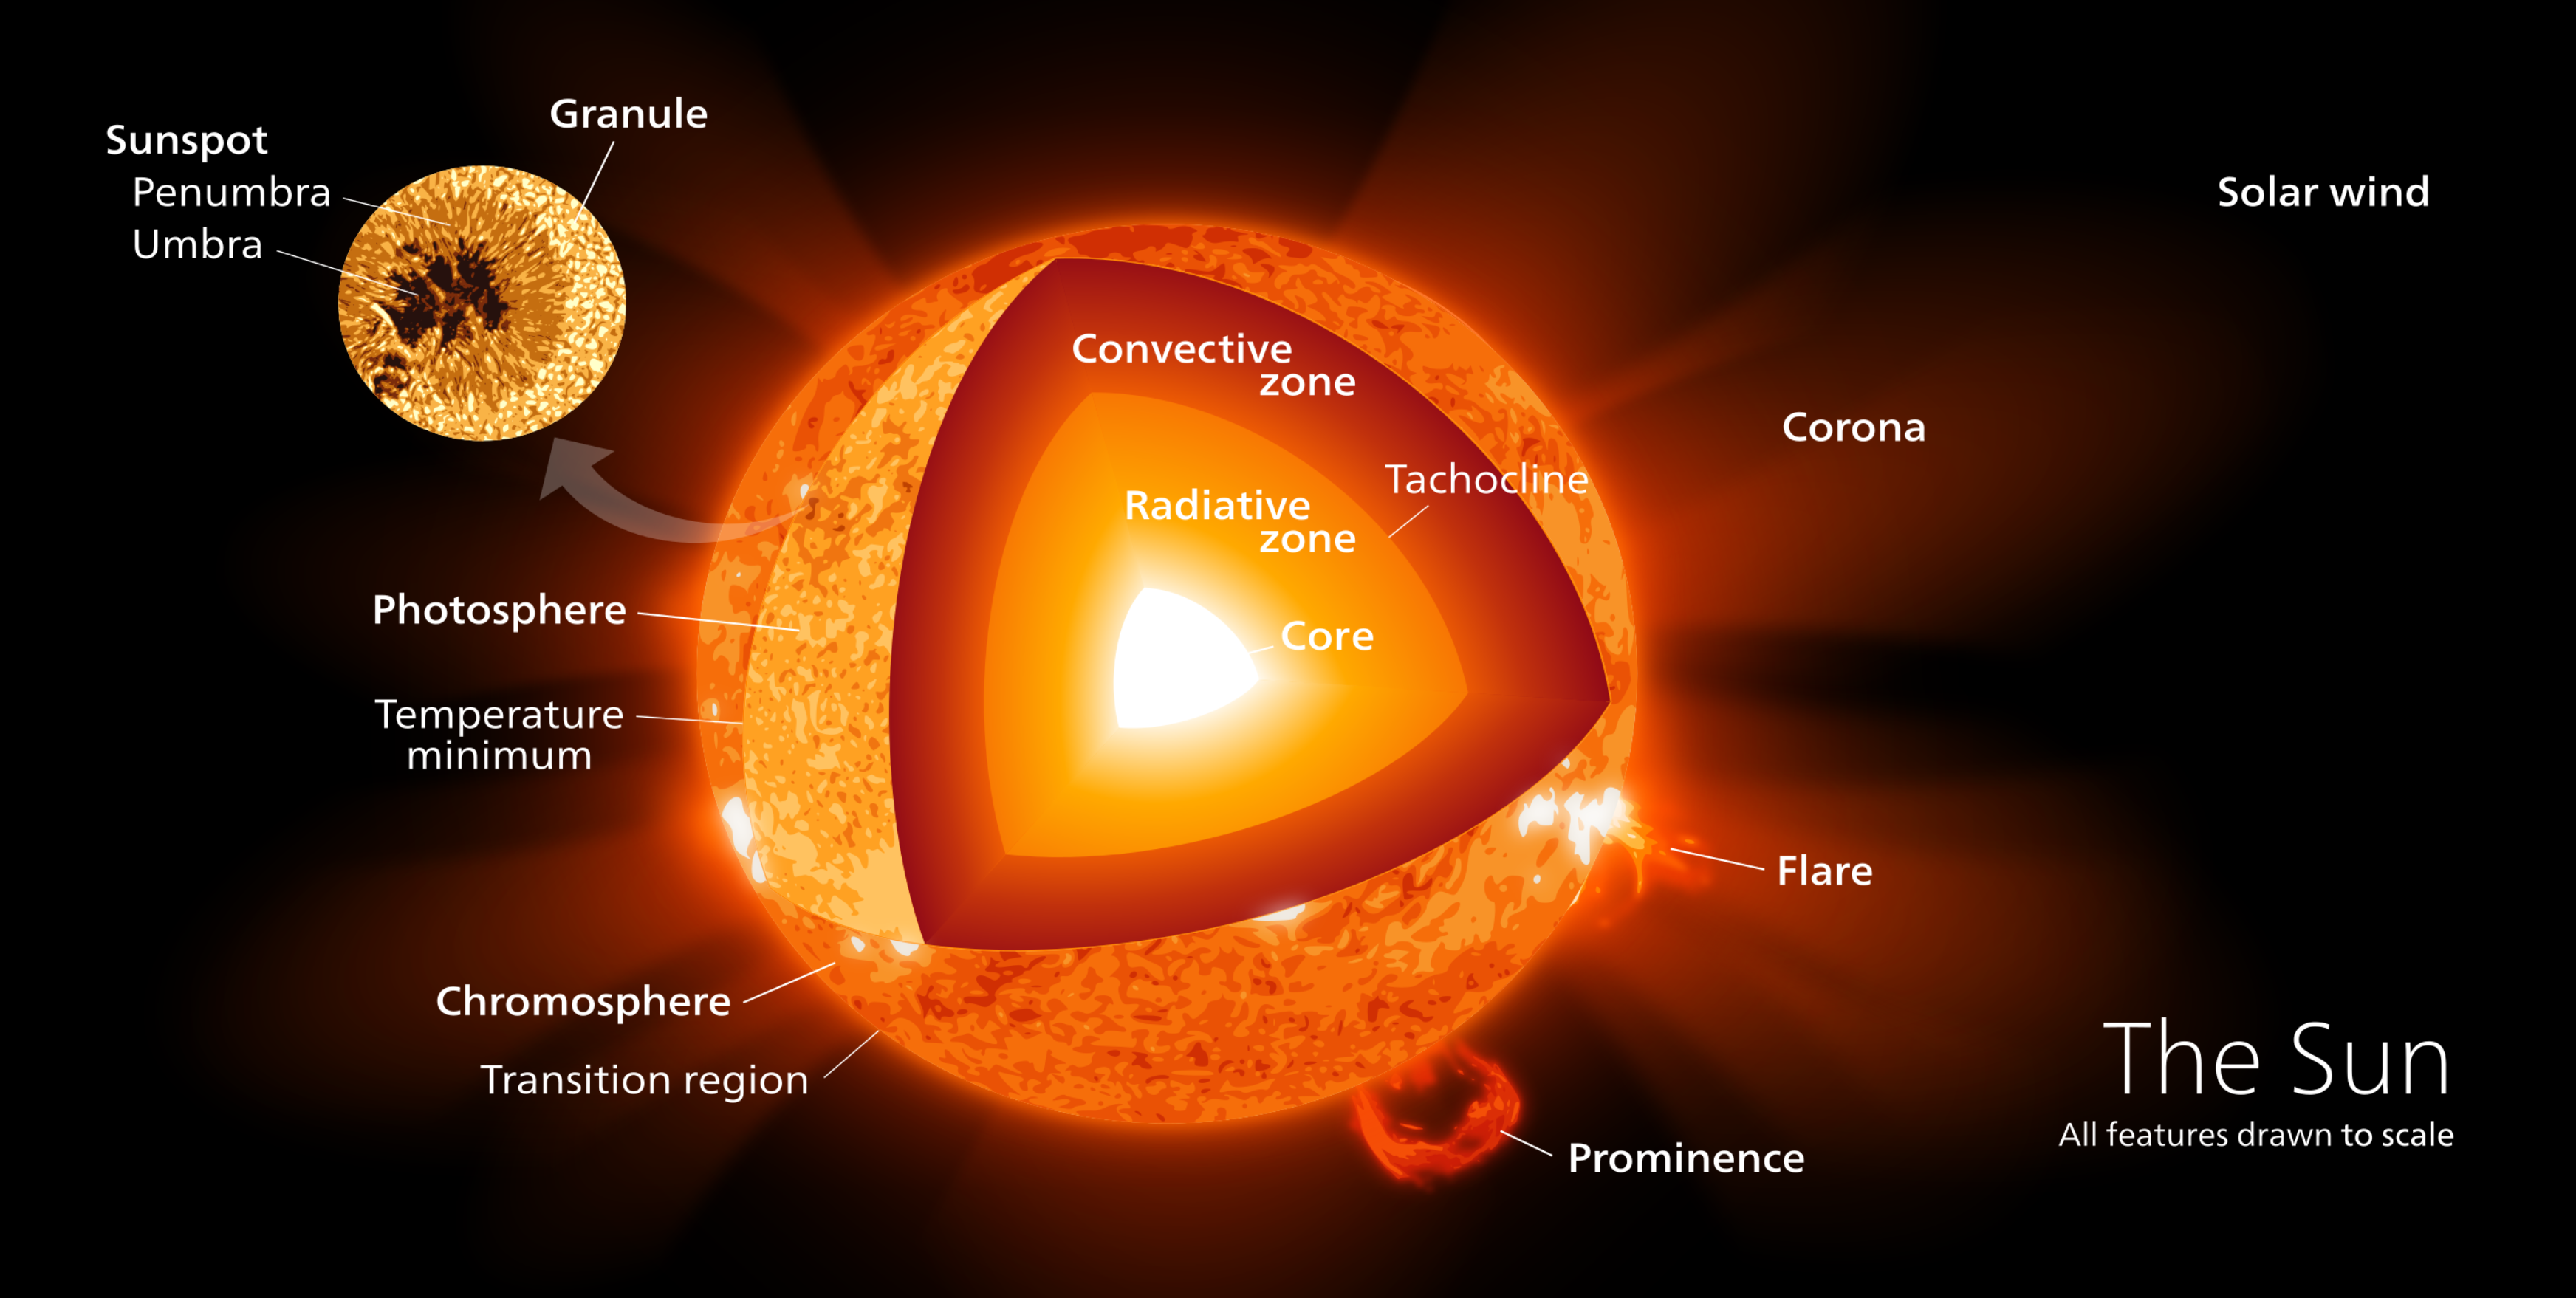
\includegraphics[width=\textwidth]{./pictures/interior.PNG}
    \caption{Visualization of the interior structure of the Sun. \cite{kelvin13}}
    \label{fig:structure}
\end{figure}
In this work we will mainly focus on phenomena related to convection, hence occurring in the convective zone and impacting photosphere.\\
Convection is the transfer of heat from one place to another by the movement of fluids. In particular, regarding the Sun, the temperature at the bottom of the convection zone is 200,000\degree K while at its outermost limit (surface of the Sun) it is being cooled by the creation of light and temperature is only about 5,700\degree K. This large difference triggers the plasma movement in order to propagate the heat outwards. Note, for instance, in Figure~\ref{fig:convect-cells} the bright regions correspond to hot rising material, whereas the dark lanes are the location where the colder material falls down into the Sun \cite{convect}. Also, as the reader can verify from Figure~\ref{fig:convect-cells}, the way convection cells organise on the surface is not regular but rather chaotic and turbulent.
\begin{figure}[t]
    \centering
    \begin{subfigure}[b]{0.49\textwidth}
        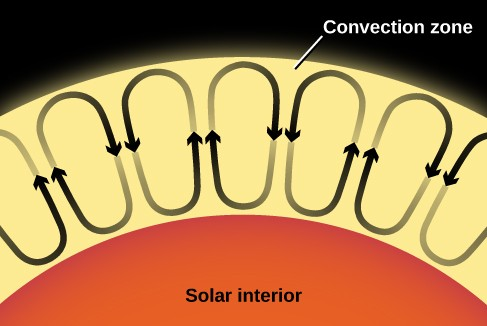
\includegraphics[width=\textwidth]{./pictures/convection}
        \caption{Section view, plasma movement}
        \label{fig:convect}
    \end{subfigure}
    \begin{subfigure}[b]{0.49\textwidth}
        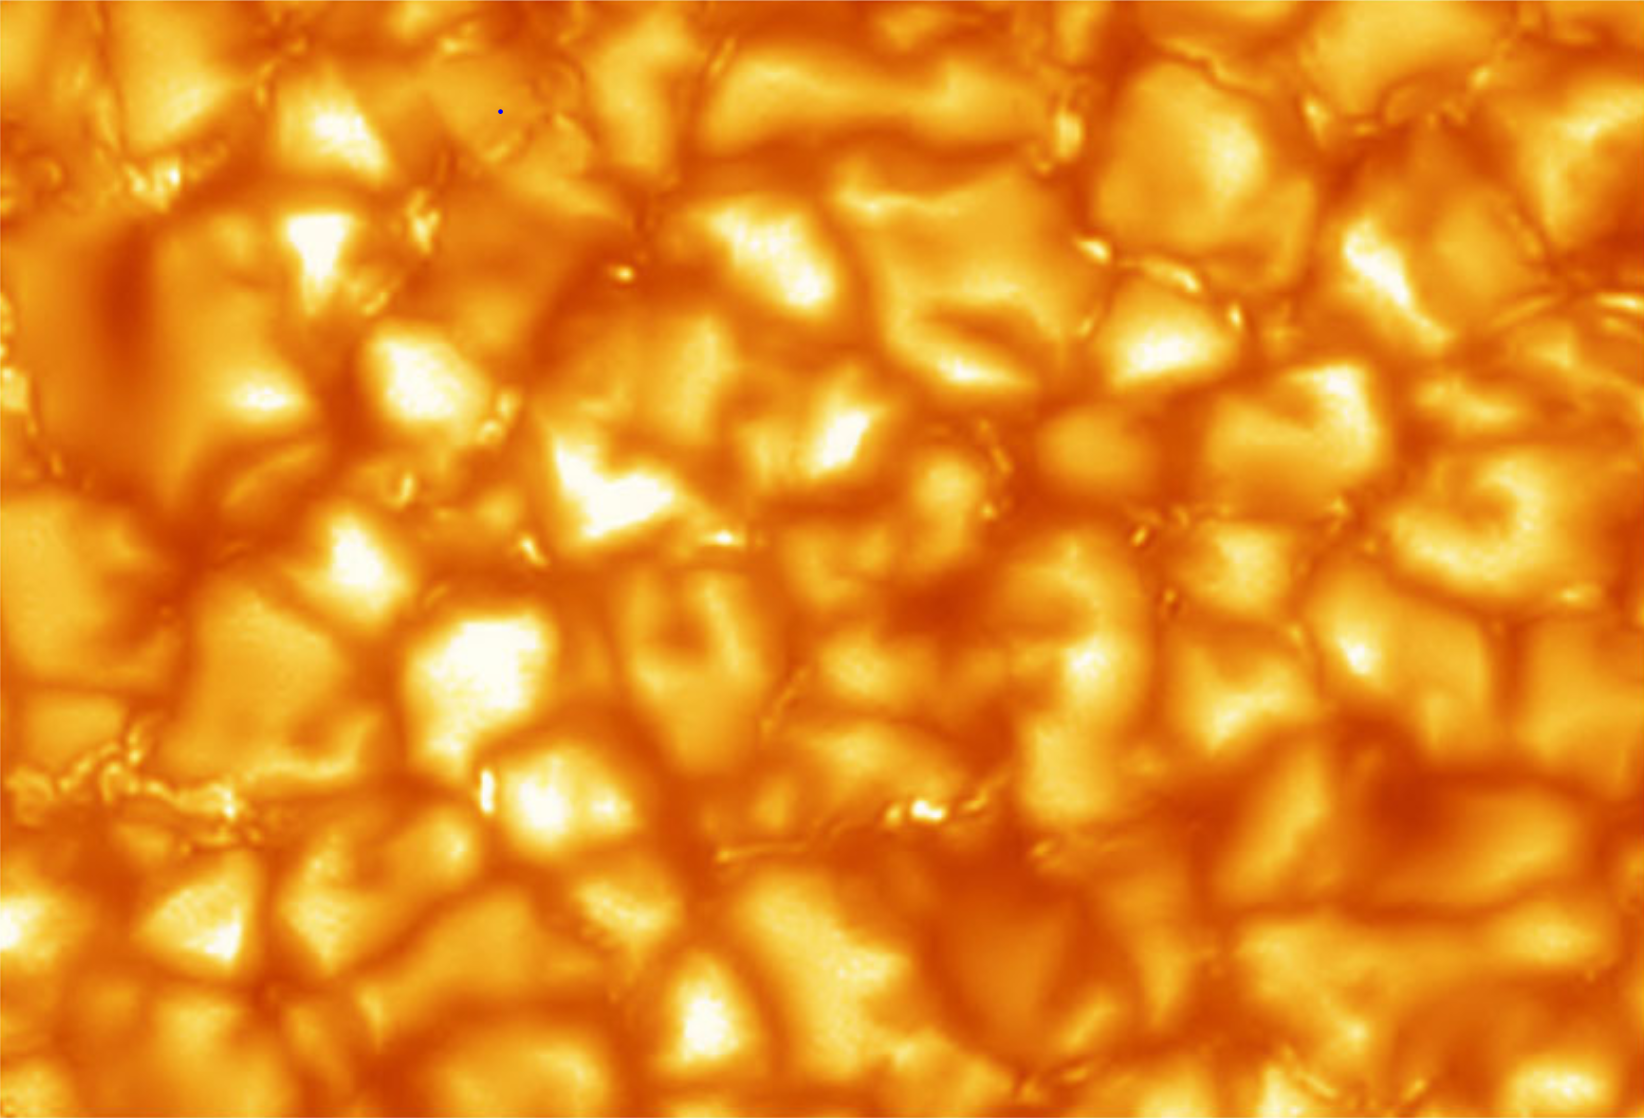
\includegraphics[width=\textwidth]{./pictures/convection-cell}
        \caption{Frontal view, convection cells.}
        \label{fig:convect-cells}
    \end{subfigure}
    \caption{Convection}\label{fig:systemview}
\end{figure}

\begin{figure}[b]
    \centering
    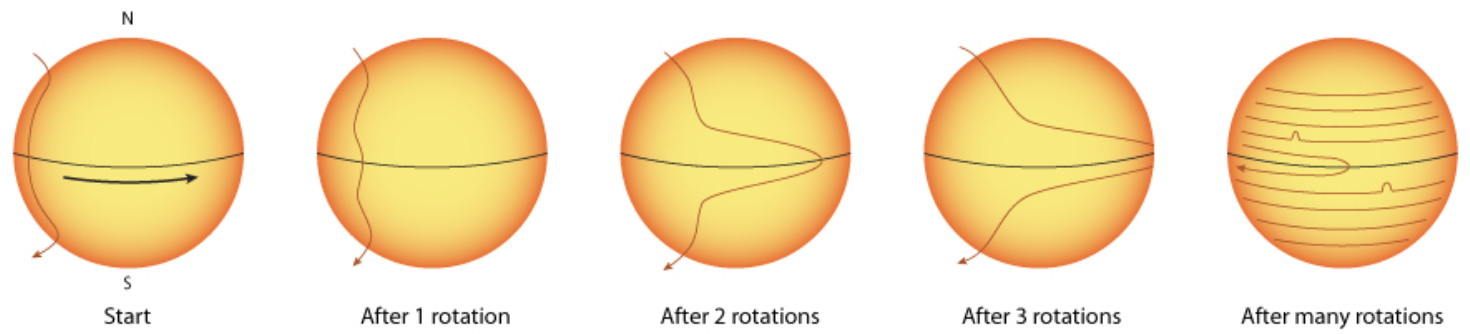
\includegraphics[width=\textwidth]{./pictures/diffrot}
    \caption{Visualization of differential rotation}
    \label{fig:diffrot}
\end{figure}
\begin{figure}[t]
    \centering
    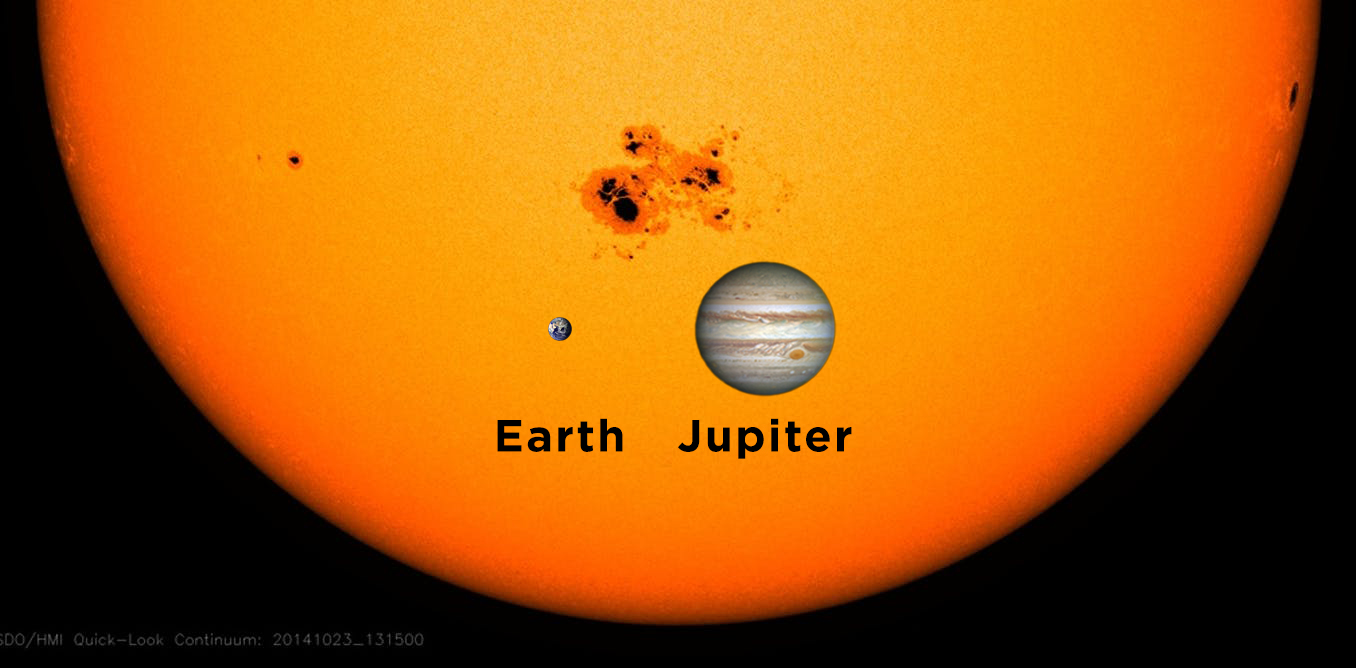
\includegraphics[width=\textwidth]{./pictures/AR12192-jup-earth}
    \caption{Relative size of AR12192, the Earth and Jupiter}
    \label{fig:AR12192-comp}
\end{figure}
Another interesting feature of the dynamics of the Sun is its rotation. In fact the Sun does not rotate uniformly, since it is not a rigid object (a solid body in which deformation is zero or very small). Our star is composed of gasses in the form of plasma and therefore the relative movement of its inner particles cannot be neglected. This results in a type of motion called differential rotation. It has been observed that the angular velocity of the particles changes in a way that depends on the latitude, in particular it is fastest on the solar equator and decreases as latitude increases \cite{diffrot}. From this notion follows that the rotation period is not constant, it takes 24.47 days at the equator and almost 38 days at the poles \cite{diffrotrev}. Furthermore this behaviour has a critical importance for the understanding of this work for two reasons. First, the features that we studied are located on the photosphere and move with the surface of the Sun, undergoing significant deformation. Second, differential rotation together with convective turbulent motions leads to the generation of electric currents and solar magnetic field. This phenomenon is called solar dynamo and is in some way similar to the dynamo effect that generates the magnetic field of the Earth. Moreover the generated magnetic field has the property that it tends to agglomerate into bundles called magnetic flux tubes. When these tubes become strong enough to locally inhibit convection the heat coming from inside the Sun is not propagated upwards and the temperature of the surface decreases significantly. The local temperature drop makes the affected area look darker than the rest of the disk. These black patches, commonly named \textbf{sunspots}, can become very large and thus fairly easy to observe, even with amateur instrumentation. Their average size is comparable to the one of the Earth, but in some cases, when the magnetic perturbation is very strong, they can reach approximately the size of Jupiter or even more, as in the case of AR12192 (Figure~\ref{fig:AR12192-comp}), the largest group of the last solar cycle. As shown in the figure the intensity gap is not uniform, the darkest areas (\textit{umbrae}) locate where the magnetic field is perpendicular to the surface, while on the periphery of the magnetic tube the field is slightly inclined and results in a lighter color (\textit{penumbrae}). Also, it has been shown that, since they indicate intense magnetic activity, sunspots accompany secondary phenomena such as coronal loops, prominences, flares and coronal mass ejections. For this reasons they have been widely observered and studied during the last 400 years. Since the invention of the telescope \cite{king2003history} (early XVII Century) many astronomers started to notice these dark features, although they weren't quite sure about their causes. Some thought they were shadows of undiscovered planets crossing the Sun, while others believed them to be dark clouds in the Sun's atmosphere. In 1843 an amateur German astronomer named Samuel Schwabe discovered the rise and fall of yearly sunspot counts we now call the solar cycle \cite{schwabe1843solar}. Nowadays we actually know that, more in general, the solar cycle is the nearly periodic 11-year change in the Sun's activity that encompasses a multitude of phenomena, as, for example, the variable levels of solar radiation and ejection of solar material. As already discussed, the change in magnitude of the activity of our star is also visible on the Earth; for instance large geomagnetic storms leading to auroras are most common during the peak of the cycle. Soon after the discovery, in 1848, Rudolf Wolf established a relative sunspot number formulation to compare the work of different astronomers using varying equipment and methodologies, known as the Wolf (or Z\"{u}rich) sunspot number \cite{vaquero2007historical}. Such definition is still in use today and we will see how later in this chapter. Wolf succeeded in reliably reconstructing the variations in sunspot number as far as the 1755--1766 cycle, which has since been known conventionally as \textit{Cycle 1}, with all subsequent cycles numbered consecutively thereafter; at the time of writing (early 2019), we are in the final phase of \textit{Cycle 24}, although the first sunspot of \textit{Cycle 25} may have appeared in early April 2018 \cite{cycle25-1}\cite{cycle25-2} or even December 2016 \cite{cycle25-3}. Using Figure~\ref{fig:SILSO2} and Figure~\ref{fig:ssarea} the reader himself can verify that the trend is indeed periodic. The graphics exhibits peaks and valleys; a peak in the sunspot count is referred to as a time of \textit{solar maximum}, whereas a valley, a period when just few sunspots appear is called a \textit{solar minimum}.
\begin{figure}[t]
    \centering
    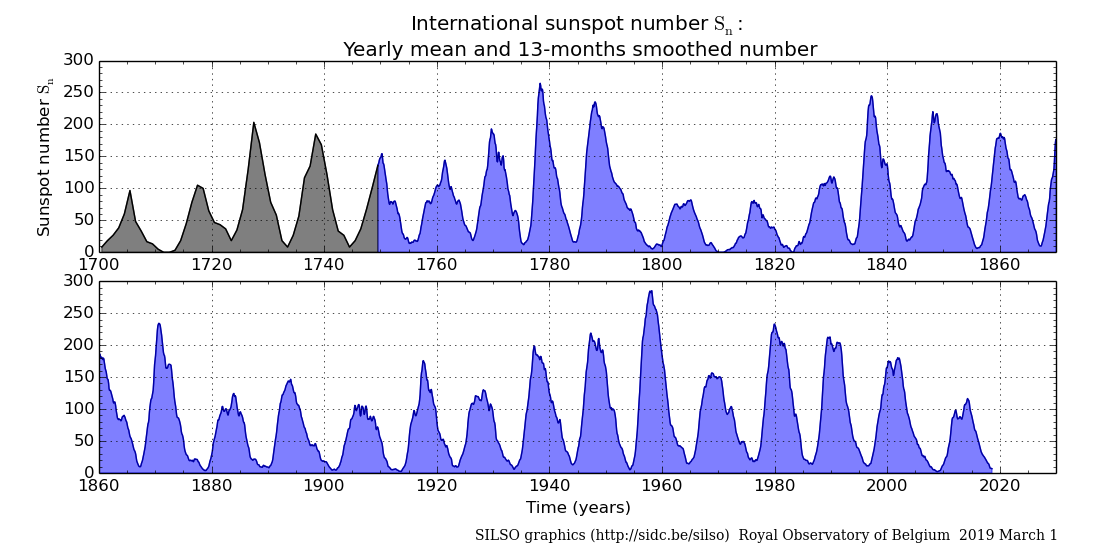
\includegraphics[width=\textwidth]{./pictures/SILSO2}
    \caption{Yearly mean sunspot number (black) up to 1749 and monthly 13-month smoothed sunspot number (blue) from 1749 up to the present.\cite{silso-graph}}
    \label{fig:SILSO2}
\end{figure}
Focusing on Figure~\ref{fig:butterfly} instead, we can discover one more property of the sunspot cycle: \textit{Sp\"{o}rer's law} \cite{ivanov2014sporer}. Sp\"{o}rer's law predicts the variation of sunspot position during a cycle by introducing the concept of \textit{cycle latitude phase} (CLP), that is calculated from the average latitudes of each sunspot over a period of time. It turns out that sunspots tend to appear around 30\degree  to 45\degree  latitude on the Sun's surface. As the cycle progresses, sunspots appear at lower and lower latitudes, until they average 15\degree  at solar maximum. The average latitude of sunspots then continues to decrease, down to about less than 10\degree  and then while the old sunspot cycle fades, sunspots of the new cycle start appearing at high latitudes. The reason why this happens is still not completely understood by the scientists.
\begin{figure}[t]
    \centering
    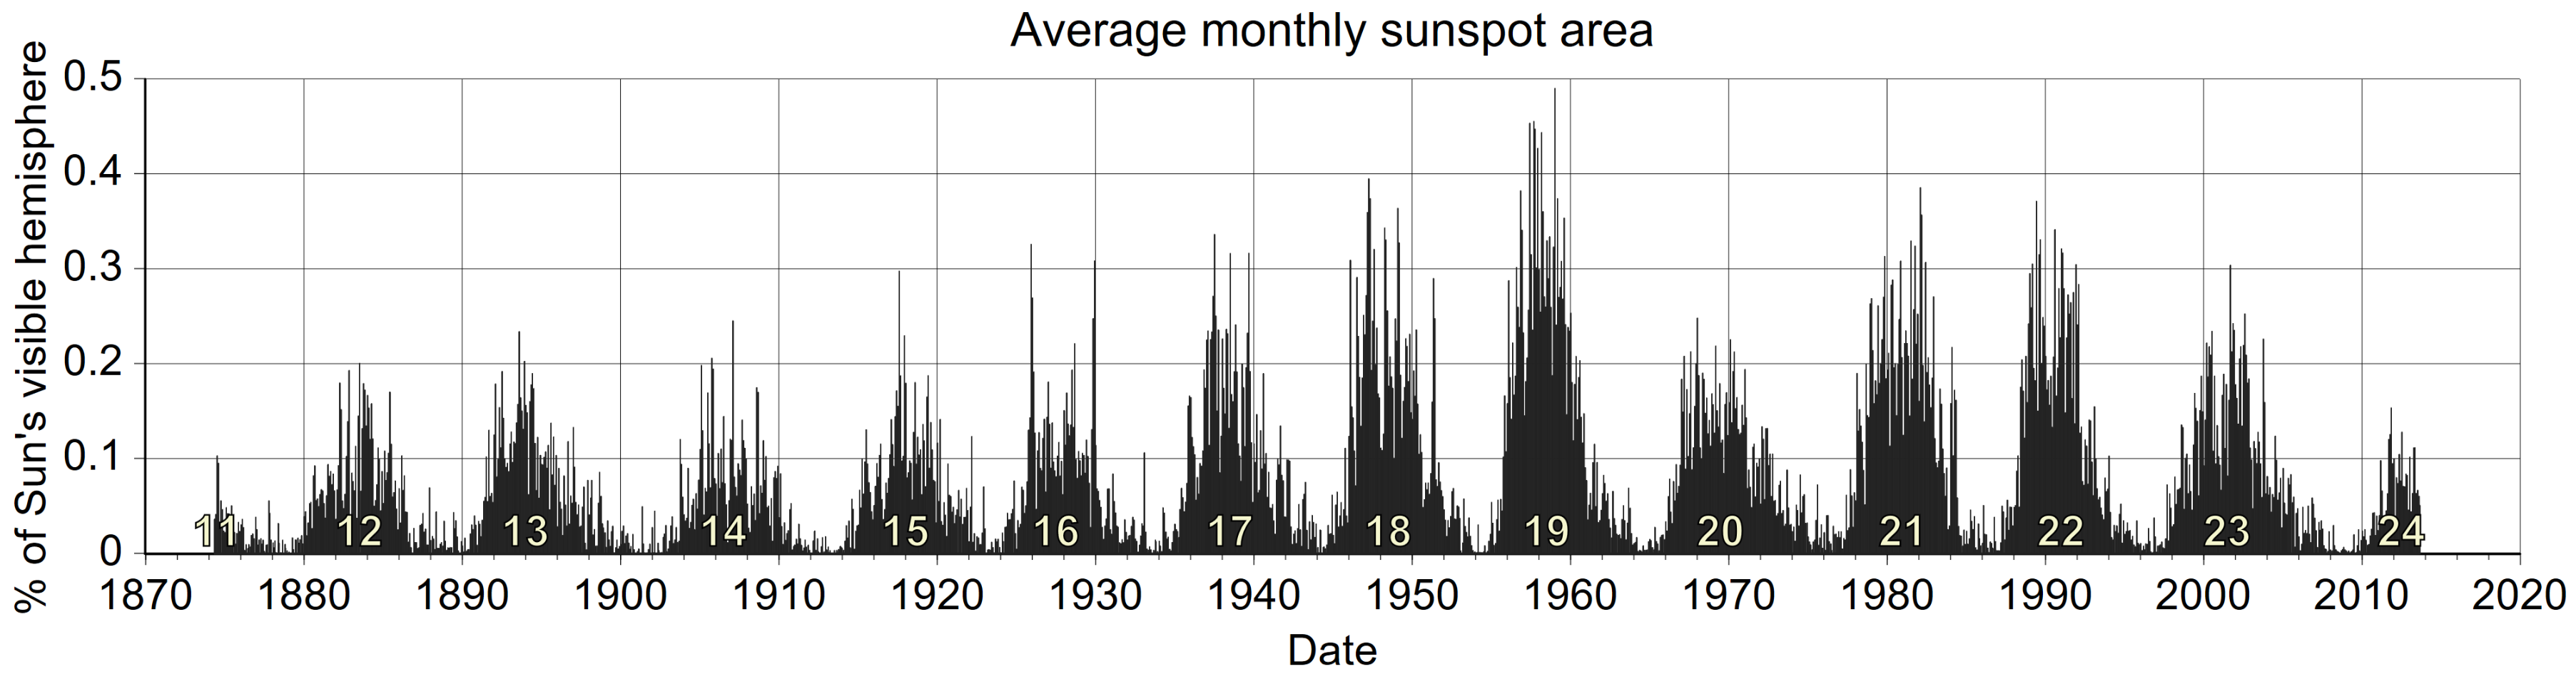
\includegraphics[width=\textwidth]{./pictures/ssarea}
    \caption{Diagram showing average monthly sunspot area from cycle 12 to cycle 24}
    \label{fig:ssarea}
\end{figure}
\begin{figure}[t]
    \centering
    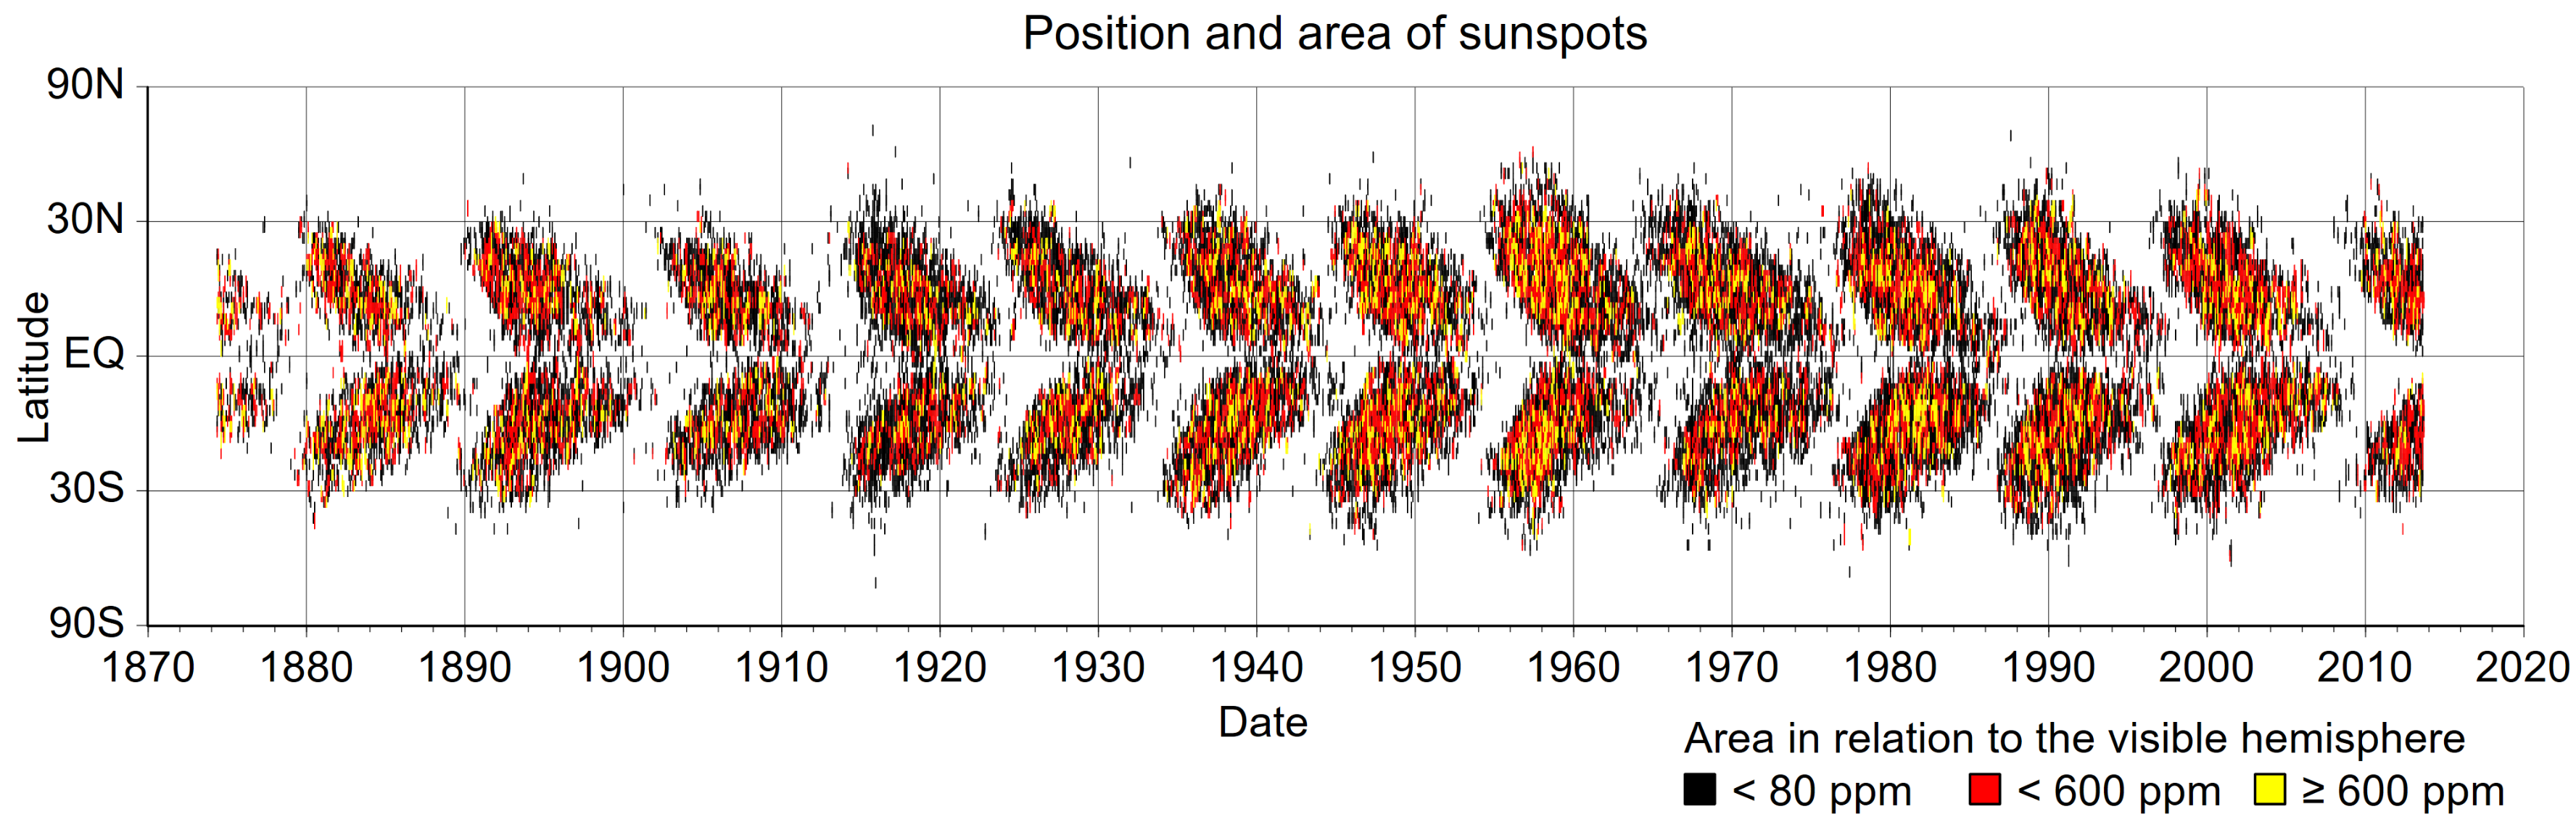
\includegraphics[width=\textwidth]{./pictures/butterfly}
    \caption{Butterfly diagram showing paired position and area of sunspots}
    \label{fig:butterfly}
\end{figure}
Another notion we need to introduce in order for the reader to fully understand this work is sunspot group classification. Several different categorization paradigms have appeared during the years but the one that is most popular nowadays is the \textit{McIntosh classification}, introduced in 1990 \cite{mcintosh1990classification}. The McIntosh classification is constituted by three components, in which the nomenclature used for each sunspot group type is \textbf{Zpc}, where Z corresponds to the \textit{Modified Z\"{u}rich Classification} and the other two components, p and c, reflect the main sunspot characteristics: the type, size, and symmetry of the penumbra and umbra; and the degree of compactness of the group \cite{carrasco2015equivalence}. We will focus on the \textbf{Z} component, that partitions the groups in the following categories\cite{silso-class}:
\begin{itemize}
  \item \textbf{A}: a small single unipolar sunspot. Representing either the formative or final stage of evolution;
  \item \textbf{B}: a bipolar sunspot group with no penumbra on any of the spots;
  \item \textbf{C}: a bipolar sunspot group. One sunspot must have penumbra;
  \item \textbf{D}: a bipolar sunspot group with penumbra on both ends of the group. Longitudinal extent does not exceed 10\degree;
  \item \textbf{E}: a bipolar sunspot group with penumbra on both ends. Longitudinal extent exceeds 10\degree  but not 15\degree;
  \item \textbf{F}: an elongated bipolar sunspot group with penumbra on both ends. Longitudinal extent of penumbra exceeds 15\degree;
  \item \textbf{H}: a unipolar sunspot group with penumbra.
\end{itemize}
Example images for each and every one of the classes can be found in Appendix 2.\\
As already described, sunspots and therefore groups are highly correlated with perturbations of the magnetic field of the Sun. In fact, besides being physically close to each other, sunspots belonging to the same groups are usually manifestations of the same \textit{active region}. These are areas of intense magnetic activity that can sometimes cause solar flares and coronal mass ejections. They are observable in several different bands of the spectrum emitted by the Sun, though normally detected using the high-energy ultraviolet band or line-of-sight (LOS) magnetograms. In general, there is a lot of research going on in multi-wavelength solar analysis, that is the field that investigates the Sun interpolating knowledge among different wavelengths. These studies are also pushed forward by the modern instrumentation we possess. Nowadays spotting active regions is pretty easy and can be achieved with several different tools (refer to Chapter 2 for more information). Once every active region is recognised it is fairly easy to determine which sunspot belongs to which group. Still, the notion of sunspot group was born a long time before active regions were observed for the first time. To clarify this, it is sufficient to think that the relationship between sunspots and magnetic field is a relatively recent finding and magnetographs only appeared at the beginning of 20th Century. However this doesn't mean that all the studies that were carried out before the invention of sophisticated space telescopes should be dismissed as ``outdated''. The complexity of modern instrumentation makes their lifespan limited and the dataset they produce quite unique. On the contrary, ground-based observatories have been pointing at the Sun during more than 400 years making it one of the longest scientific experiment in the human history. Longevity makes it possible to capture secular variability and therefore enabling long-term analysis that wouldn't be possible otherwise. Sure enough, ground observation has its own limitations as well. Despite being very stable in the long term it can't be considered reliable in short periods of time. In fact, considering a single observatory as source of data, it is impossible to estimate the daily number of sunspots consistently. This happens because the quality of the data is strongly affected by the dynamics of the atmosphere. If the thick layer of air that sits inbetween the telescope and the Sun is turbulent or hazy the resulting images will loose definition, intruducing a bias on the sunspot count. On the other hand, if the atmosphere is quiet and transparent the light will travel without trouble, making the obseravtions almost as good as the ones of space telescopes. It is understood that if the solar disk is obscured by the clouds during the whole day the counting is impossible and it should be regarded as a missing data point. Nowadays, to overcome these limitations the SIDC/SILSO \cite{sidc-silso}, the most important authority in the field, uses an ensemble of hundreds of observatories to produce the sunspot number series \cite{Clette2015}. Averaging over several heterogeneous detections has many benefits, namely: mitigating the variance, improving accuracy and solving missing data problems. However, it also introduces a new layer of complexity in the computation of the final index, since it is not possible to perform a simple average considering that the available stations are different from day to day. Every set-up has its own, unique properties that should be taken into account in the calculation. Luckily, this uniqueness is already captured in the personal reduction coefficient ($K$) included in the \textit{relative sunspot number} formula by R. Wolf:
\begin{equation}\label{relssnum}
R = K \cdot (10 \cdot g + s)
\end{equation}
The way this solar activity index is calculated hasn't changed much since its establishment, 400 years ago. What changed, though, is our ability to resolve very small spots on the surface of the Sun and highlight them through post-processing. \\
An example of the processing techniques that can help scientists in the counting is \textit{limb darkening correction}. This method consists in the reduction of the phenomenon of limb darkening through software. This phenomenon is an optical effect intrinsic to the physics of the observation, that causes an imbalance in the quantity of photons we receive from the limb of the disk compared to its center (refer to Figure~\ref{fig:AR12192-comp} for a visual intuition). In practice, this can be pleasant to the eye because it gives the viewer the idea of the sphericity of the Sun, but it is also inconvenient when trying to detect small features on the edge. The theoretical laws that govern the magnitude of the darkening for each point of the surface are very rich and interesting but they are out of the scope of this thesis. In any case, there are much simpler solutions that are able to correct the images only leveraging the intensity profile of the image (more details will be given in Chapter 3). Other interesting post-processing techniques for feature enhancement will be illustrated in Appendix 3, including for instance gradient sharpening, off-limb emission enhancement and mean intensity correction. \\
Finally, to conclude this brief introduction to solar physics, it is necessary to present some basic aspects of the large topic of \textit{solar coordinate systems}. Standardizing the way the position of solar features is encoded is vital for the creation of large scale datasets, but at the same time it is very difficult for several reason. The first reason is that the axis of rotation of our star is tilted with respect to the ecliptic of the Earth. Therefore the solar north pole, as seen from the our planet, appears displaced. Clearly, the displacement is not constant, but rather periodic. As the Earth procedes on its orbital path, the observed axial tilt changes in a range that goes from -7\degree to 7\degree. The second reason that should be considered in the study of solar coordinates is that the Sun is a gaseous body, there are no fixed points of reference and this is made worse by differential rotation. Moreover it is also not perfectly spherical, although its oblateness is rather small and almost neglectable \cite{dicke1974oblateness}. The last reason is represented by the fact that the revolution and rotation of the Earth itself influences our perspective of the Sun. For this reason, a coordinate should not really be considered complete if it doesn't include time. The deveopment of sophisticated coordinate systems for solar image data allows to overcome, at least partially, these difficulties. Nowadays, solar coordinate systems can be divided into 3 categories \cite{thompson2006coordinate}:
\begin{enumerate}
  \item \textbf{Heliographic Coordinates}: latitude and longitude of a feature are expressed on the solar surface, and can be extended to three dimensions by adding the radial distance from the center of the Sun. There are two basic variations on the heliographic system: \textbf{Stonyhurst} and \textbf{Carrington} heliographic. Both use the same solar rotational axis (based on the original work by R. Carrington in 1863), and differ only by an offset in the longitude definition.
  \item \textbf{Heliocentric Coordinates}: any system of coordinates where the origin of the axes is located at the centre of the Sun. The system can be \textbf{cartesian}, when the z axis is defined to be parallel to the observer-Sun line and the y axis points towards the north pole, or \textbf{radial} if it uses a position angle measured from the projection of the north pole and a radial distance.
  \item \textbf{Helioprojective Coordinates}: observations are projected against the celestial sphere and all projective angles have origin at disk center, considered as the apparent disk center as seen by the observer without any corrections made for light travel time or aberrations.
\end{enumerate}



% \begin{figure}[b]
%     \centering
%     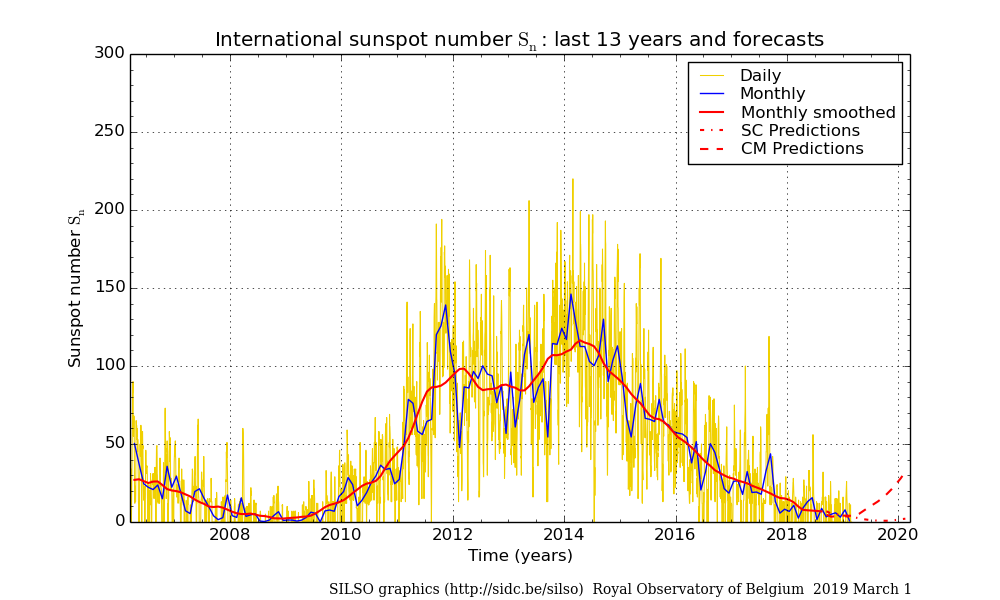
\includegraphics[width=\textwidth]{./pictures/SILSO1}
%     \caption{Daily sunspot number (yellow), monthly mean sunspot number (blue), smoothed monthly sunspot number (red) for the last 13 years and 12-month ahead predictions of the monthly smoothed sunspot number. SC = prediction method based on an interpolation of Waldmeier's standard curves. CM = method (from K. Denkmayr and P. Cugnon) combining a regression technique applied to the sunspot number series with the a geomagnetic index used as a precursor}
%     \label{fig:SILSO1}
% \end{figure}
%
%
% \begin{figure}[t]
%     \centering
%     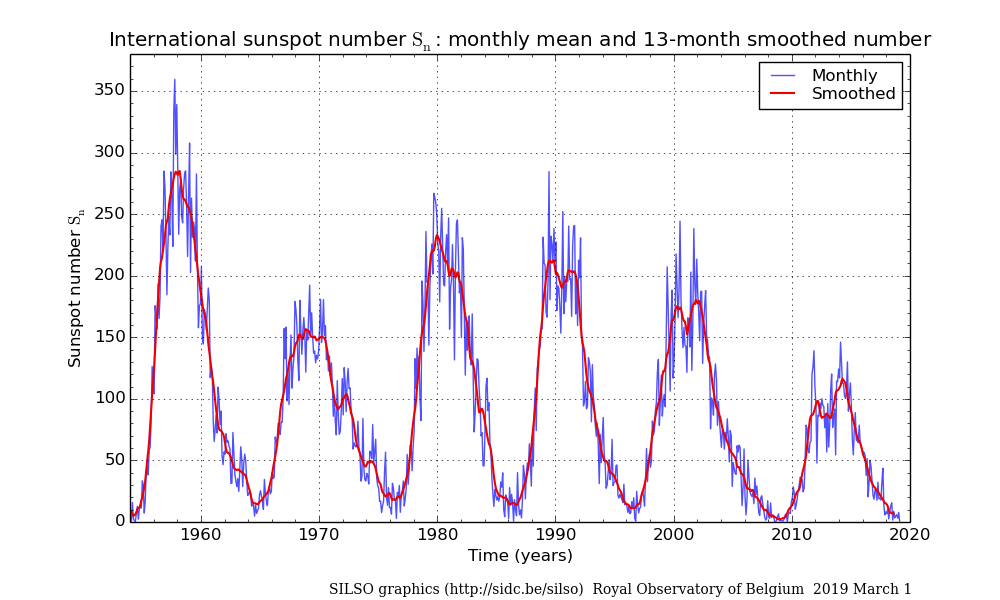
\includegraphics[width=\textwidth]{./pictures/SILSO3}
%     \caption{The monthly mean sunspot number (blue) and 13-month smoothed monthly sunspot number (red) for the last five cycles.}
%     \label{fig:SILSO3}
% \end{figure}

% \begin{figure}[t]
%     \centering
%     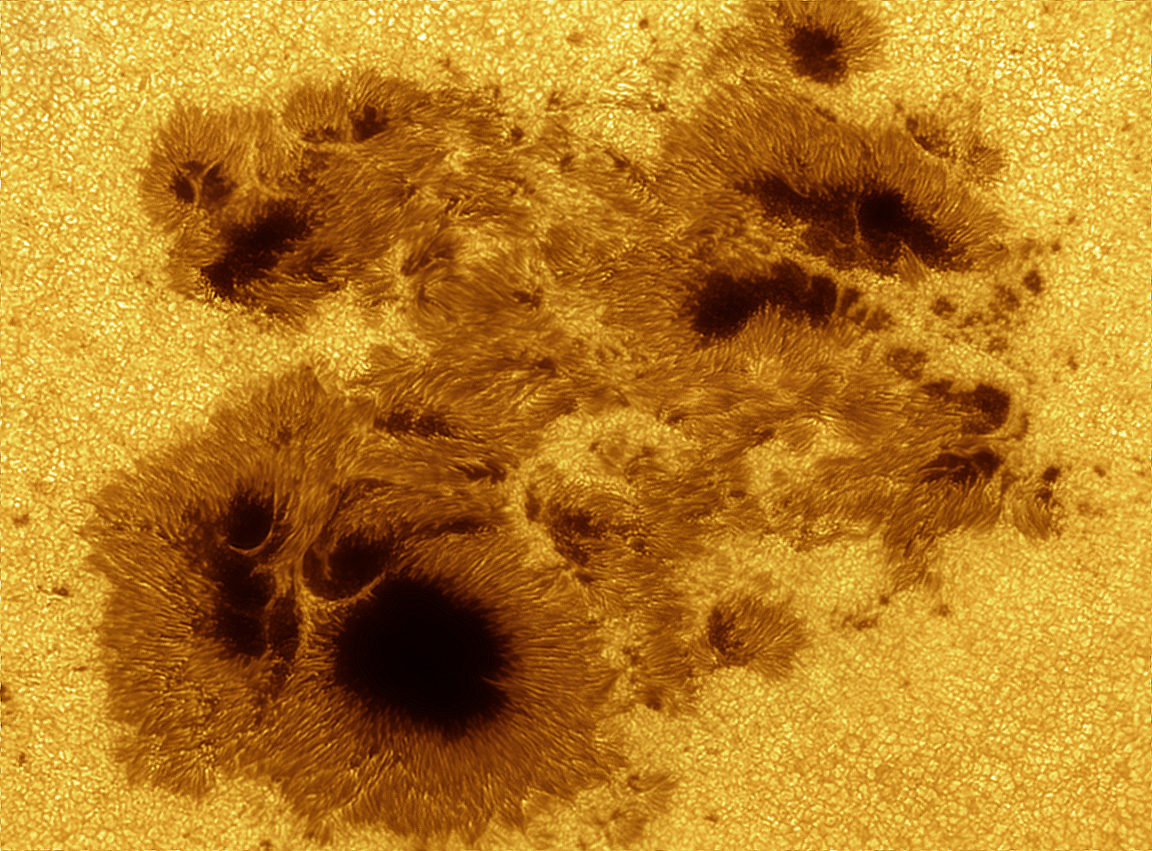
\includegraphics[width=\textwidth]{./pictures/AR12192}
%     \caption{Close up picture of AR12192}
%     \label{fig:AR12192}
% \end{figure}
